\chapter{Theoretische Grundlagen und Verwandte Arbeiten}
In diesem Kapitel werden grundlegende Begriffe erklärt, die für das Verständnis der Arbeit unabdingbar sind.

\section{Containerisierung}
Containerisierung ist eine Technik, den Code einer Anwendung mitsamt aller Abhängigkeiten, die zur deren Ausführung benötigt werden, zu verpacken. Ein solches Paket wird als Container-Image bezeichnet. Da alle Abhängigkeiten enthalten sind, werden dadurch die Laufzeitunterschiede auf unterschiedlichen Plattformen minimiert\cite{noauthor_what_nodate}. Zur Laufzeit wird ein Container-Image als Container bezeichnet. Um ein Container-Image auszuführen, wird eine Container-Runtime benötigt. Die erste Container Runtime-Engine wurde von Docker entwickelt, wird aber mittlerweile als Open-Source Projekt mit dem Namen containerd von der Open Container Initiative (OCI) betrieben\cite{noauthor_what_nodate}. 

Containerisierte Anwendungen unterscheiden sich von Virtuellen Maschinen vor allem darin, dass kein Hypervisor zur Ausführung der Images benötigt wird. Stattdessen teilen sich alle Container das Host-Betriebssystem und werden in einem eigenen User-Space isoliert. Dadurch sind Container-Images deutlich leichtgewichtiger und können schneller als Virtuelle Maschinen ausgeführt werden\cite{noauthor_what_nodate}. Abbildung \ref{fig:containerVsVMs} verdeutlicht nochmals den Unterschied beider Technologien.

\begin{figure}[H]
    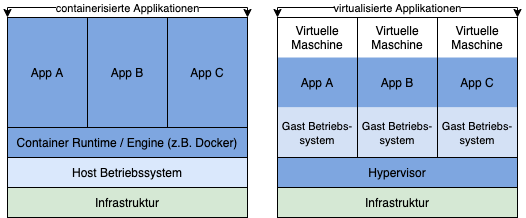
\includegraphics[width=\textwidth]{img/container-vs-vms.png}
    
    \caption[Vergleich zwischen Containern und Virtuellen Maschinen]{Vergleich zwischen Containern und Virtuellen Maschinen (angelehnt an: \cite{noauthor_what_nodate})}
    \label{fig:containerVsVMs}
\end{figure}

\section{Container-Orchestrierung}
Container-Orchestrierung beschreibt die Automatisierung der \linebreak "`Bereitstellung, Verwaltung, Skalierung und Vernetzung von Containern"'\cite{noauthor_was_nodate}. Mit Orchestrierungs-Tools lassen sich Container einfach auf Computer-\linebreak Clustern provisionieren, skalieren und überwachen. Sie ermöglichen das Betreiben von infrastrukturunabhängigen und flexiblen Anwendungen auf Basis von Containern\cite{noauthor_was_nodate-1}. Beispiele für bekannte Orchestrierungs-Tools sind Kubernetes oder \ac{ECS}, welcher in dieser Arbeit verwendet wird.

\section{Serverless}
Serverless ist ein Software-Ausführungsmodell, bei dem ein Cloud Anbieter (z.B \ac{AWS}, Microsoft Azure, \ac{GCP}) sich vollständig um die Ausführung einer Anwendung inklusive Konfiguration der zugrundeliegenden Server und deren Skalierung kümmert. Ein Programmierer von Serverless-Anwendungen kann sich daher ausschließlich auf das Schreiben des Codes konzentrieren und muss keine Zeit in das Einstellen und Aufsetzen von Servern investieren\cite{ken_owens_cncf_2018}. 

Serverless Anwendungen werden grundlegend unterschieden in \ac{FaaS} und \ac{BaaS}; wobei es sich bei letzterem um API-basierte, automatisch skalierte Services von Drittanbietern handelt, die grundlegende Bausteine einer Applikation ersetzen\cite{ken_owens_cncf_2018}. Beispiele für \ac{BaaS} sind \ac{S3} als Speicher von Dateien oder \ac{AWS} DynamoDB als NoSQL-Datenbank.

In dieser Arbeit sollen ausschließlich \ac{FaaS} betrachtet werden. Bei diesem Ausführungsmodell wird die Software in einem Stateless-Container, d.h einem Container ohne persistentem Speicher, ausgeführt. Der Cloud-Anbieter stellt dabei die Ressourcen dynamisch bzw. on-demand bereit, d.h die Anwendung wird nur dann ausgeführt, wenn eine diesbezügliche Anfrage, also eine Ereignis, eintrifft. Serverless verspricht dadurch eine effizientere Entwicklung und Kosteneinsparungen, da von den Anbietern nur der tatsächlich laufenden Code abgerechnet wird\cite{noauthor_was_2016}. 

\section{AWS Lambda}
Die in dieser Arbeit getestete Serverless-Anwendung wird auf Lambda, einem \ac{FaaS}-Angebot von \ac{AWS}, ausgeführt. Die Funktionsweise des Lambda-Services lässt sich wie folgt beschreiben (alle Informationen dieser Sektion basieren auf dem \ac{AWS} Lambda Entwicklerhandbuch\cite{amazon_aws_aws_2020}):

\begin{enumerate}
\item Es tritt ein Event ein, dass die Ausführung der Lambda-Funktion anfordert. \\
    Dabei kann es sich um eines von vielen möglichen Ereignissen handeln, bspw. ein Dateiupload in \ac{S3}, einen CRON-Job oder, im Falle eines Web-Backends, ein API-Aufruf durch ein API-Gateway.

\item Init Phase: Lambda erstellt automatisch eine Ausführungsumgebung (environment). \\
    Dabei handelt es sich um eine isolierte Umgebung, die für die Ausführung der Lambda- Funktion benötigt wird. Für diese Umgebung lassen sich einige Parameter vom Anwender konfigurieren:
    
    \begin{enumerate}
        \item Die Runtime: Dabei handelt es sich um die verwendete Programmiersprache bzw. das verwendete Framework. Als Optionen bietet Lambda beispielsweise Node.js, Java, Python oder Go an.
        \item Die Arbeitsspeichergröße: Sie bestimmt, wie viel Speicher der ausgeführten Funktion bereitsteht. Die Mindestgröße beträgt hier \linebreak 128 Megabyte. Maximal sind etwas mehr als 10 Gigabyte möglich. Proportional zur Speichergröße legt Lambda ebenfalls die CPU-Leistung fest, mit der die Funktion ausgeführt wird.
        \item Timeout: Die maximale Ausführungszeit der Funktion bevor Lambda sie automatisch beendet. Hier sind maximal 15 Minuten möglich.
    \end{enumerate}
    
    Die Umgebung wird mit den konfigurierten Ressourcen (Arbeitsspeicher und CPU) erstellt, der Code der Funktion aus \ac{S3} in den Funktions-Container geladen und entpackt und der Initialisierungscode (nicht die Funktion an sich) ausgeführt. An dieser Stelle lässt sich bspw. eine Datenbankverbindung aufbauen.
    
\item Invoke Phase: In dieser Phase wird die eigentliche Lambda-Funktion, welche auch als Handler bezeichnet wird, ausgeführt. Eventuelle Rückgabewerte werden an den Aufrufer zurückgeliefert. Nachdem der Handler ausgeführt wurde, bleibt er verfügbar für weitere Anfragen. Der Initialisierungscode wird allerdings nicht mehr ausgeführt.
    
\item Shutdown Phase: Nachdem die Funktion für einige Zeit nicht mehr angefragt wurde, wird die Ausführungsumgebung wieder freigegeben. 
\end{enumerate}

\begin{figure}[H]
    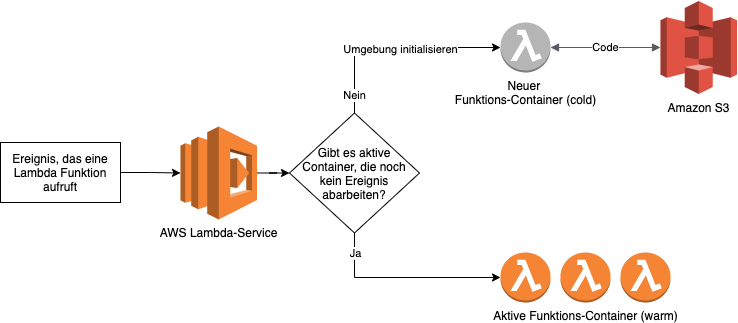
\includegraphics[width=\textwidth]{img/lambda-architecture.png}
    
    \caption[AWS Lambda Funktionsweise]{AWS Lambda Funktionsweise (angelehnt an: \cite{noauthor_serverless_2017})}
    \label{fig:lambda-architecture}
\end{figure}

\subsection{Cold- und Warmstart}
Nachdem der Handler in der Invoke-Phase ausgeführt wurde, wird die Ausführungsumgebung nicht sofort wieder freigegeben, sondern für einige Zeit vorgehalten, um weitere Anfragen schneller zu bearbeiten. Dies wird auch als Warmstart bezeichnet, da die Runtime-Umgebung bereits initialisiert ist und der Handler sofort aktiviert werden kann.
Muss die Umgebung nach einer eingetroffenen Anfrage erst noch initialisiert werden, also zunächst die Init-Phase ausgeführt werden, wird dies als Coldstart bezeichnet. Aufgrund des Mehraufwandes, erweist sich ein Coldstart als deutlich langsamer als ein Warmstart. 

\subsection{Nebenläufigkeit}
Befindet sich der Handler einer Lambda-Funktion gerade in der Ausführung und es trifft ein weiteres Ereignis ein, startet Lambda zusätzlich zu der bereits laufenden Funktion eine weitere Ausführungsumgebung, um diese neue Anfrage zu verarbeiten. Da nun mehrere Umgebungen gleichzeitig ausgeführt werden, wird dies auch als Nebenläufigkeit (engl. concurrency) bezeichnet. Bei vielen gleichzeitigen Anfragen werden also so viele Umgebungen wie nötig erstellt. Der \ac{AWS} Lambda-Service erlaubt standardmäßig 1.000 nebenläufige Funktionen pro Region, dieser Wert lässt sich allerdings nach Absprache mit \ac{AWS} erhöhen.

Treten vermehrt Anfragen in kürzerer Zeit auf, werden automatisch neue Instanzen aufgesetzt, die diese bearbeiten können. Bereits initialisierte Umgebungen werden wiederverwendet. Lässt die Nachfrage nach, werden Umgebungen automatisch wieder heruntergefahren. Abbildung \ref{fig:lambda-architecture} verdeutlicht nochmals den gesamten Prozess, in dem Lambda neue Funktions-Container erstellt oder bereits gestartete wiederverwendet.